\documentclass[a4paper,ngerman]{scrartcl}

\usepackage{amsmath}
\usepackage{amsfonts}
\usepackage{amssymb}
\usepackage[utf8]{inputenc}
\usepackage{graphicx}
\usepackage[ngerman]{babel}
\usepackage{hyperref}
\usepackage{float}
\usepackage{caption}
\usepackage{subcaption}
\usepackage{multirow}  %for tables
\usepackage{icomma} % Handle german comma as decimal point in numbers
\usepackage{units,siunitx} % Write units with correct spacing
\usepackage{upgreek} % provide non-italic greek letters
\usepackage{url}


% Formatting of table & figure captions
\captionsetup{font={sf,footnotesize},labelfont=bf,textfont=sl,skip=6pt}
\setlength{\abovecaptionskip}{6pt}
\setlength{\belowcaptionskip}{0pt}

\title{Quantenradierer}
\date{\today}
\author{Michel Rausch, Michael Eliachevitch}

\begin{document}

\maketitle
\tableofcontents
\thispagestyle{empty} % remove page number from abstract page
\newpage
\setcounter{page}{1}






\section{Theoretische Überlegungen}
\label{sec:theorie}

\subsection{Interferenz von Wellen, klassisch und quantenmechanisch}
\label{sec:interferenz}

\subsection{"`Welcher-Weg"'-Information}
\label{sec:welcher-weg}


\clearpage
\section{Das Mach-Zehnder-Interferometer und dessen Aufbau}
\label{sec:mach-zehnder}

\subsection{Aufbau eines einfachen Interferometers}
\label{ssec:interferomter-einfach}

Die theoretischen Überlegungen können in Interferometern geprüft werden. In einem einfachem Strahlteilungsinterferometer, wie in Abbildung \ref{fig: Interferometer-einfach} gezeigt. Eine planare Welle, hier Licht, wird mit einem halbtransparentem Spiegel in Wellen A und B aufgeteilt. Der Strahl A (rot im Bild) passiert den Strahlteiler und das Interferometer. Der zweite wird über Spiegel umgelenkt und erhält so eine längere Laufzeit, mit Gangunterschied $\Delta z$. Am zweiten Strahlteiler rekombinieren die Wellen. Dies wurde in \ref{sec:interferenz} beschrieben.

\begin{figure}
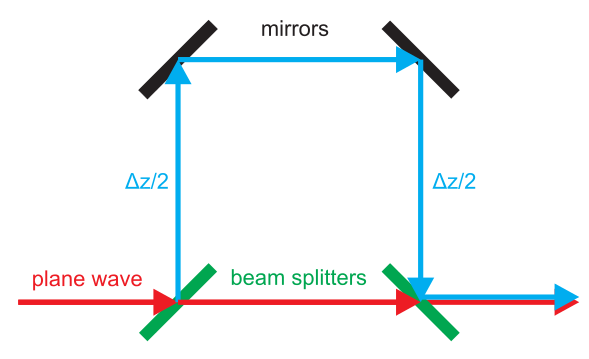
\includegraphics[width=0.5\textwidth]{interferomter-einfach.png}
\caption{Einfaches Interferometer, zur Strahlteilung und -rekombination, mit dem Laufzeitunterschied $\Delta z$ [\ref{ref:mappe}]}
\label{fig: Interferometer-einfach}
\end{figure}

\subsection{Quantenradierer}
\label{ssec:quantenradierer}

In diesen Versuch wird das Mach-Zehnder 

\begin{figure}
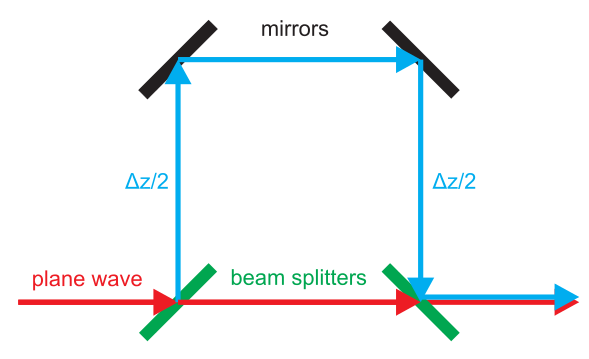
\includegraphics[width=0.5\textwidth]{interferomter-einfach.png}
\caption{Skizze eines Mach-Zehnder-Interferomters mit Polarisatoren ($45^{\circ}$ und $-45^{\circ}$) [\ref{ref:mappe}]}
\label{fig:mach-zehnder}
\end{figure}



\section{Versuchsdurchführung}
\label{sec:versuchsdurchfuhrung}


\clearpage
\section{Quellen}
\begin{enumerate}
\item Vorbereitungsmappe \label{ref:mappe}
\end{enumerate}



\end{document}
